\chapter{Results} \label{chap:results}

\begin{chapquote}{\textit{Thomas Huxley}}
``The great tragedy of science is the slaying of a beautiful hypothesis by an ugly fact.''
\end{chapquote}

This chapter contains the main experimental findings and results of LCMs. Section \ref{sec:exp-setup} elaborates on the experimental setup for assessing the performance of trained models. Section \ref{sec:metrics} is dedicated to the definition of the evaluation metrics for LCMs, while Section \ref{sec:baselines} contains the selection and description of established benchmarks. Section \ref{sec:ablations} concerns low to medium-scale results of ablation studies, while Section \ref{sec:res-lcms} covers results of large-scale LCMs. Trained models are evaluated on various dataset collections, both synthetic and simulated, as well as on in-distribution and out-of-distribution settings.


\section{Evaluation Setup} \label{sec:exp-setup}

Our evaluation setup can be briefly described as follows: We generate data collections as described in Chapter \ref{chap:data}, train LCMs with varying capabilities as described in Chapter \ref{chap:architecture} and using a training protocol as in Chapter \ref{chap:training}. We assess their predictive capabilities on various data collections, synthetic, semi-synthetic and simulated, both in-distribution and out-of-distribution, using performance metrics described in Section \ref{sec:metrics}.  

\section{Measuring Causal Discovery Performance} \label{sec:metrics}

We select standard metrics for predictive performance, as well as for causal graph distance. We evaluate the inferred lagged causal graph \(\hat{G}\) based on the presence and absence of directed edges compared to the ground truth lagged causal graph \(\mathcal{G}\). Recall that both the ground truth and inferred lagged causal graphs are padded both in the variable and lag dimension, so comparison is done on these padded graphs. Since causality is an asymmetric measure, and furthermore in the temporal case edges move forward in time, the directionality of an edge is taken into account.  We evaluate the learnt edges in terms of True Positives (TP), False Positives (FP), True Negatives (TN) and False Negatives (FN) \citep{sokolova2009systematic}. Ultimately, our comparisons revolve around the Area under the ROC curve (AUC) \citep{bradley1997use} metric, which is the reported metric in the main text. Their known definitions are applied, but for comparing the edges on the ground truth and inferred lagged causal graphs (Table \ref{tab:metrics}).

\begin{table}[ht!]
\centering
\caption{Definitions of evaluation metrics for binary predictions on learned causal graphs.}
\label{tab:metrics}
\begin{tabular}{ll}
\textbf{Metric} & \textbf{Definition} \\ \hline
TPR & Proportion of positives correctly identified. \\[6pt]
FPR & Proportion of negatives incorrectly identified as positives. \\[6pt]
TNR & Proportion of negatives correctly identified. \\[6pt]
FNR & Proportion of positives incorrectly identified as negatives. \\[6pt]
Precision & Proportion of positives correctly identified. \\[6pt]
Recall & Proportion of positives correctly identified. \\[6pt]
F1 & Harmonic mean of precision and recall. \\[6pt]
\textbf{AUC} & Area under the ROC curve (TPR vs. FPR) across different thresholds.
\end{tabular}
\end{table}

\par{TPR, FPR, TNR, FNR}. The \textit{True Positive Rate (TPR)} (also known as \textit{sensitivity}) measures the proportion of actual positives that are correctly identified by the model. \( \text{TPR} = \frac{TP}{TP + FN} \). The \textit{False Positive Rate (FPR)} measures the proportion of actual negatives that are incorrectly identified as positives, \( \text{FPR} = \frac{FP}{FP + TN} \). The \textit{True Negative Rate (TNR)} (also known as \textit{Specificity}), measures the proportion of actual negatives that are correctly identified as negatives, \( \text{TNR} = \frac{TN}{TN + FP} \). Finally, the \textit{False Negative Rate (FNR)} measures the proportion of true edges that are incorrectly identified as non-existent, \( \text{FNR} = \frac{FN}{FN + TP} \).

\par{Precision, Recall, F1}. We Additionally measure the \textit{Precision} (also known as \textit{Positive Predictive Value}) and \textit{Recall} (also known as \textit{Sensitivity}) metrics, which are defined as \(\text{Precision} = \frac{TP}{TP + FP}\), \(\text{Recall} = \frac{TP}{TP + FN}\) and \(\text{F1} = \frac{2 \cdot \text{Precision} \cdot \text{Recall}}{\text{Precision} + \text{Recall}}\). 

\par{AUC}. We measure the AUC (Area under ROC Curve) \citep{bradley1997use} using the area under the True Positive Rate and False Positive Rate at different prediction thresholds, based on the adjacency tensors of the ground truth and predicted DAGs. This is the same metric as the adjacency-based AUC introduced in Section \ref{sec:sim-results}, referred here simply as \(\mathrm{AUC}\). The predicted probabilities are obtained from the model and thresholded to \(\tau=0.05\), as well as the ground truth adjacencies (labels). Both time-lagged adjacency tensors are then flattened and concatenated along their batch dimension.

Figure \ref{fig:lagged-causal-graphs} depicts an example of a metric comparison between the ground truth and a possibly inferred output graph. 

\begin{figure}[t!]
\centering

% --- (a) Ground Truth ---
\begin{minipage}[t]{0.48\textwidth}
\centering
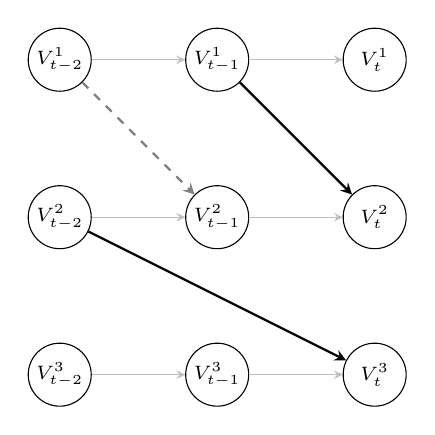
\begin{tikzpicture}[
    every node/.style={draw, circle, minimum size=0.8cm, font=\scriptsize, inner sep=0pt},
    >=stealth,
    ->,
    dashededge/.style={->, dashed, thick, color=gray},
    solidedge/.style={->, thick},
]

% t-2
\node (V1t2) at (0,4) {$V^1_{t-2}$};
\node (V2t2) at (0,2) {$V^2_{t-2}$};
\node (V3t2) at (0,0) {$V^3_{t-2}$};

% t-1
\node (V1t1) at (2,4) {$V^1_{t-1}$};
\node (V2t1) at (2,2) {$V^2_{t-1}$};
\node (V3t1) at (2,0) {$V^3_{t-1}$};

% t
\node (V1t) at (4,4) {$V^1_{t}$};
\node (V2t) at (4,2) {$V^2_{t}$};
\node (V3t) at (4,0) {$V^3_{t}$};

% Temporal arrows
\foreach \i in {1,2,3} {
  \draw[->, gray!50] (V\i t2) -- (V\i t1);
  \draw[->, gray!50] (V\i t1) -- (V\i t);
}

% Causal arrows (Ground truth)
\draw[solidedge] (V1t1) -- (V2t);
\draw[dashededge] (V1t2) -- (V2t1);
\draw[solidedge] (V2t2) -- (V3t);

\end{tikzpicture}

\vspace{0.3em}
{(a) Ground Truth}
\end{minipage}
\hfill
% --- (b) Inferred Graph ---
\begin{minipage}[t]{0.48\textwidth}
\centering
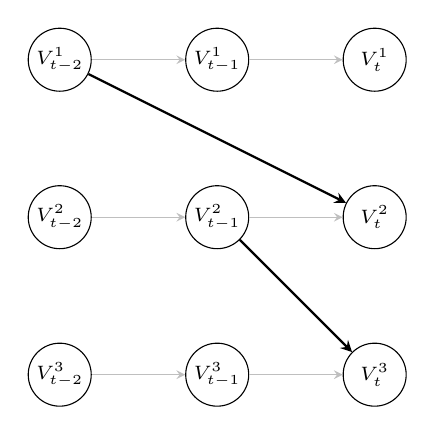
\begin{tikzpicture}[
    every node/.style={draw, circle, minimum size=0.8cm, font=\scriptsize, inner sep=0pt},
    >=stealth,
    ->,
    dashededge/.style={->, dashed, thick, color=gray},
    solidedge/.style={->, thick},
]

% t-2
\node (V1t2) at (0,4) {$V^1_{t-2}$};
\node (V2t2) at (0,2) {$V^2_{t-2}$};
\node (V3t2) at (0,0) {$V^3_{t-2}$};

% t-1
\node (V1t1) at (2,4) {$V^1_{t-1}$};
\node (V2t1) at (2,2) {$V^2_{t-1}$};
\node (V3t1) at (2,0) {$V^3_{t-1}$};

% t
\node (V1t) at (4,4) {$V^1_{t}$};
\node (V2t) at (4,2) {$V^2_{t}$};
\node (V3t) at (4,0) {$V^3_{t}$};

% Temporal arrows
\foreach \i in {1,2,3} {
  \draw[->, gray!50] (V\i t2) -- (V\i t1);
  \draw[->, gray!50] (V\i t1) -- (V\i t);
}

% Causal arrows (Inferred Example)
\draw[solidedge] (V1t2) -- (V2t);   % Wrong lag
\draw[solidedge] (V2t1) -- (V3t);   % Found one
% Missed edge: (V1t1 -> V2t)

\end{tikzpicture}

\vspace{0.3em}
{(b) Inferred Example}
\end{minipage}

\caption{Ground truth vs. inferred lagged causal graph with \(\ell_{\max}=2\) and \(3\) variables. Dashed edges encode causal stationarity, solid edges denote direct causal influence.}
\label{fig:lagged-causal-graphs}
\end{figure}

Although LCMs output a soft adjacency tensor \(\hat{\mathbb{A}}\) as discussed in Section \ref{sec:problem-formulation}, obtaining a binary causal graph from the soft predictions requires some sort of thresholding to the confidence scores. A thresholding operator is therefore defined, \(\hat{\mathcal{G}} = 1\{\hat{\mathbb{A}} \geq \tau\}\), with \(\tau\) either fixed (e.g., \(\tau = 0.05\)) or varied to compute ROC and AUC. Unless otherwise specified, reported results use \(\tau=0.05\). This procedure separates the training objective (which operates directly on soft predictions) from the evaluation protocol (which relies on binarized graphs). For threshold-independent comparisons, we sweep \(\tau\) to compute ROC and AUC.

\section{Comparison with Existing Approaches} \label{sec:baselines}

We compare the results of our framework with three other established works\footnote{For an overview on causal discovery algorithms, we refer the reader to the review paper by \citet{niu2024comprehensive}.} for temporal causal discovery: 

\begin{enumerate}

  \item The Peter-Clark Momentary Conditional Independence (\textit{PCMCI}) is a time-series causal discovery algorithm introduced by \cite{runge2018causal}. It is based on the constraint-based Peter-Clark (PC) algorithm by \cite{spirtes2001causation}, uncovering causal relationships using conditional independence tests of the form \( X_i(t-\tau) \rightarrow X_j(t) \) for lag \( \tau=0,\ldots,\ell_\text{max} \). The algorithm assumes the causal Markov condition, faithfulness, causal stationarity and causal sufficiency, while also accounting for contemporaneous (\(\tau=0\)) causation. The process consists of two phases, (i) the PC phase where, starting from a fully connected time-lagged graph up to lag \(\ell_\text{max}\) iteratively prunes spurious relationships by testing conditional independences, given a conditioning set and (ii) the MCI phase where, using Momentary Conditional Independence, tests for causal relationships while conditioning on both lagged and contemporaneous variables. Specifically, for each remaining candidate edge \(X^i_{t-\tau} \to X^j_t\), the Momentary Conditional Independence (MCI) test is performed, conditioning on both past and contemporaneous parents of \(X^j_t\) and parents of \(X^i_{t-\tau}\). This reduces false positives caused by autocorrelation and contemporaneous confounding, yielding higher precision in estimated causal graphs. In our implementations we use the official implementation of PCMCI, available in the \texttt{Tigramite} Python package. We select \(\alpha=0.05\) as the threshold of the adjacency matrix's p-values exclude contemporaneous edges, \( \ell_\text{max} = 3\). For independence tests we utilize partial correlation, which is estimated through a linear Ordinary Least Squares (OLS) regression and testing for non-zero linear Pearson correlation on the residuals and GPDC, which is a  conditional independence test based on Gaussian processes and distance correlation.

  \item \textit{DYNOTEARS} \citep{pamfil2020dynotears} is a time-series causal discovery algorithm, viewed as an extension of the NOTEARS \citep{zheng2018dags} method, which introduced causal discovery as a mathematical optimization problem with smooth acyclicity constraint. By leveraging the trace exponential function to enforce acyclicity and promoting sparsity using the \(\ell_1\) norm, this optimization program is solved using the augmented Lagrangian method, translating it into a series of unconstrained problems, in a similar setup to NOTEARS. Assuming \( M \) independent realizations of a \textit{stationary} time-series \( \left\{ x_{m,t} \right\}_{t=0}^{T} \) for \(\mathbf{x}_{m,t} \in \mathbb{R}^{d}\), the authors model the data using a Linear Structural Vector Autoregression (SVAR) model. The model is expressed as

  \begin{equation}
  \mathbf{x}_{m,t} = \mathbf{x}_{m,t}W + \sum_{i=1}^{p} \mathbf{x}_{m,t-i}A_i + \mathbf{z}_{m,t},
  \end{equation}

  where \(W\) represents contemporaneous (\textit{intra-slice}) dependencies, \(A_i\) lagged (\textit{inter-slice}) dependencies, and \( \mathbf{z}_{m,t} \) independent error terms. In matrix form this translates to,

  \begin{equation}
  \mathbf{X} = \mathbf{X}W + \mathbf{Y}A + \mathbf{Z},
  \end{equation}

  where \( \mathbf{X} \) contains the observations, \( \mathbf{Y} \) the time-lagged versions of \( \mathbf{X} \) and \( A \) is the concatenated matrix of lagged weights. The parameters of DYNOTEARS, apart from \( \ell_\text{max} \), are the regularization constants \(\lambda_\mathbf{W}, ~\lambda_{\mathbf{A}} \) that control the sparsity (as causal graphs are in general sparse), and the weight thresholds \(\tau_\mathbf{W}, ~\tau_{\mathbf{A}}\) that reduce the numerical error when computing \( h(\mathbf{W}) = \text{trace}(e^{\mathbf{W} \circ \mathbf{W}}) -d\). In our implementations, we select \(\lambda_{\mathbf{W}}=\lambda_{\mathbf{A}}=0.1\), thresholds \(\tau_\mathbf{W}=\tau_{\mathbf{A}}=0.05\), maximum number of iterations in the augmented Lagrangian method \(n=100\) and \(\ell_\text{max}=1\). Since DYNOTEARS' formulation is based on intra-slice and inter-slice dependencies for modeling the influence between variables in a contemporaneous and time-lagged setting respectively, we drop the contemporaneous predictions as we assume no contemporaneous effects in our experimental setup.

  \item \textit{VARLiNGAM} \citep{hyvarinen2010estimation} extends the LiNGAM (Linear Non-Gaussian Acyclic Model) to time-series data by integrating it with vector autoregressive (VAR) models and infers both lagged and contemporaneous causal relations, whereas the classic VAR only analyzes lagged causal relationships. Specifically, it estimates a Structural Vector Autoregression (SVAR) model of the form

  \begin{equation}
  \mathbf{x}(t) = \sum_{\tau=0}^{k} B_{\tau} \mathbf{x}(t-\tau) + \mathbf{e}(t),
  \end{equation}

  where \(B_\tau\) are \(n \times n\) coefficient matrices for lag \(\tau\), and \(\mathbf{e}(t)\) is a vector of mutually independent, non-Gaussian disturbances. The matrix \(B_0\) encodes instantaneous (contemporaneous) causal relations, while \(B_\tau, \, \tau>0\), encode lagged causal relations. 

  The key assumptions are: (i) linearity of the causal relations, (ii) non-Gaussianity and independence of disturbances, (iii) acyclicity of contemporaneous relations, and (iv) absence of latent confounders. Unlike Gaussian SVARs, where identifiability requires strong priors, VARLiNGAM leverages Independent Component Analysis (ICA) to achieve identifiability purely from statistical properties of the data. Estimation proceeds in two stages: first, autoregressive coefficients \(M_\tau\) are estimated via least squares; second, the residuals are subjected to LiNGAM analysis to recover instantaneous effects \(B_0\). The full causal matrices are then reconstructed as 
  
  \begin{equation}
  \hat{B}_\tau = (I - \hat{B}_0) \hat{M}_\tau, \quad \tau > 0
  \end{equation}

This yields a consistent estimator of both instantaneous and lagged effects. The authors show that neglecting \(B_0\) can severely bias lagged estimates, underscoring the importance of modeling contemporaneous effects.  In our experiments, we implement VARLiNGAM using the publicly available code and set \(\ell_\text{max}=3\), assuming first-order dependencies. Evaluation is restricted to lagged effects, discarding contemporaneous ones, in accordance with our experimental setup that excludes instantaneous causation.
 
\end{enumerate}

In addition to the above baselines, we also compare against the pre-trained Transformer model by \citet{stein2024embracing} on our 5-dimensional evaluation datasets.

\begin{algorithm}[t]
\caption{Bootstrap-based Estimation of Edge Probabilities} \label{alg:bootstrap}
\begin{algorithmic}[1]
\REQUIRE Time-series dataset $\mathcal{D}$, maximum lag $\ell_{\max}$, number of bootstraps $n$, causal discovery algorithm configuration $\mathbf{B}_\text{CD}$
\ENSURE Soft adjacency matrix $\mathbb{A} \in [0,1]^{V \times V \times \ell_{\max}}$

\STATE Initialize accumulator $\mathbf{S} \gets \mathbb{0}^{V \times V \times \ell_{\max}}$

\FOR{$b = 1$ to $n$}
    \STATE \COMMENT{Bootstrap Sampling Phase}
    \STATE Draw bootstrap sample $\mathcal{D}^{(b)}$ from $\mathcal{D}$ by resampling with replacement

    \STATE \COMMENT{Causal Discovery Phase}
    \STATE $\mathbf{A}^{(b)} \gets \text{causalAlg}(\mathcal{D}^{(b)}, \mathbf{B}_\text{CD})$

    \STATE \COMMENT{Edge Confidence Update}
    \STATE $\mathbf{S} \gets \mathbf{S} + f(\mathbf{A}^{(b)})$ 
    \STATE \COMMENT{$f$ extracts edge indicators or confidence scores}
\ENDFOR

\STATE \COMMENT{Normalization Phase}
\STATE $\mathbf{A} \gets \mathbf{S} / n$

\RETURN $\mathbf{A}$
\end{algorithmic}
\end{algorithm}

For all baselines, the official implementations are used or adapted, where needed, and the inferred graphs are transformed into a lagged adjacency form to ensure a fair comparison. The lag hyperparameter \(\ell_\text{max}\) is set precisely to that of our LCMs, i.e. \(\ell_\text{max}=3\). It should further be noted that not all methods output a lagged adjacency matrix of probabilities for edge existence (confidence scores) like our LCMs. For constraint-based methods like PCMCI, we use the inverse of the edge p-values as confidence scores, since the method outputs the p-values of the conditional independence tests for each lagged edge. For models that output an adjacency matrix of causal effect coefficients (like VARLiNGAM and DYNOTEARS), results are not directly comparable to our LCMs that output soft adjacency probabilities and computing AUCs is not directly applicable. For a fair comparison, we follow a bootstrap-based procedure to estimate the probability of each causal edge, as shown in the official documentation\footnote{\url{https://lingam.readthedocs.io/en/latest/tutorial/var.html}}. Specifically, we run both VARLiNGAM and DYNOTEARS \(n=10\) times with resampled datasets and compute the proportion of times each edge is discovered, resulting in a soft adjacency matrix of edge probabilities. Although computationally expensive, this approach allows for The pseudocode for this approach is shown in Algorithm \ref{alg:bootstrap}. 

To assess whether the differences in AUC scores between not only LCMs but benchmark methods as well are statistically significant, we employ the \textit{Wilcoxon signed-rank test}, a non-parametric paired test suitable for non-normally distributed data such as AUC scores. To control the family-wise error rate from multiple comparisons, we apply the \textit{Bonferroni correction} \(\alpha_\text{corrected} = \frac{\alpha}{k} \) where \(k\) is the number of pairwise comparisons. Additionally, each dataset instance is evaluated \(10\) times with different random seeds to obtain standard errors and confidence intervals. In the main text, the mean \(\mathrm{AUC}\) is reported (as defined in Section \ref{sec:metrics}) with standard errors. A complete list of experimental results is provided in the Appendix. 

\section{Ablation Studies} \label{sec:ablations}

\subsection{Ablation on Training Aid Techniques} \label{sec:ablation-training-aids}

In Chapters \ref{chap:architecture} and \ref{chap:training}, two approaches for enhancing the performance of LCMs were presented, as introduced by \citet{stein2024embracing}: \textit{Correlation Injection (CI)} (Subsection \ref{subsec:ci}) and \textit{Correlation Regularization (CR)} (Subsection \ref{subsec:cr}). The impact of both techniques is now quantitatively and thoroughly evaluated in terms of causal discovery performance, a gap that was previously unfilled. We report results for medium-sized LCMs (\(\approx 1\)M parameters) trained on the \texttt{S\_Joint} collection (Subsection \ref{subsec:data-training-synth}, Table \ref{tab:synthetic-datasets}) for in-distribution testing.

A baseline LCM was trained without any training aids, a second variant with CI only, and several models combining CI and CR with a grid search over the space of weight coefficients \(\lambda_{\text{CR}} \in \{0.25, 0.5, 0.75, 1.0\}\). The objective was two-fold: (i) to assess the relative contributions of CI and CR, and (ii) to identify a stable \(\lambda_{\text{CR}}\) value for subsequent large-scale experiments.

\begin{table}[h]
\centering
\caption{Ablation of training aids on \texttt{S\_Joint} (in-distribution). Statistical significance refers to improvement over the preceding variant, under a Bonferroni correction for multiple comparisons.}
\label{tab:training_aids_ablation}
\small
\begin{tabular}{lcc}
\toprule
\textbf{Model} & \textbf{AUC} & \textbf{Significant} \\
\midrule
LCM & 0.830 {\tiny $\pm$ .000} & -- \\
LCM + CI & 0.845 {\tiny $\pm$ .000} & Yes \\
LCM + CI + CR, ($\lambda_{CR}=0.25$) & 0.870 {\tiny $\pm$ .000} & Yes \\
LCM + CI + CR, ($\lambda_{CR}=0.5$) & 0.876 {\tiny $\pm$ .000} & Yes \\
LCM + CI + CR, ($\lambda_{CR}=0.75$) & 0.875 {\tiny $\pm$ .000} & No (vs 1.0) \\
LCM + CI + CR, ($\lambda_{CR}=1.0$) & 0.875 {\tiny $\pm$ .000} & No (vs 0.75) \\
\bottomrule
\end{tabular}
\end{table}

Table \ref{tab:training_aids_ablation} illustrates that both CI and CR substantially enhance causal discovery accuracy. CI alone provides a statistically significant improvement over the baseline (\(p < 10^{-7}\)), while the addition of CR further increases AUC across all tested regularization strengths. The highest mean AUC (\(0.876\)) is achieved for \(\lambda_{\text{CR}} \in [0.5, 0.75]\), with negligible variance.

A post-hoc significance analysis (Table \ref{app:training-aids-ablation-significance} in the Appendix) confirms no statistically significant difference between \(\lambda_{\text{CR}}=0.75\) and \(\lambda_{\text{CR}}=1.0\) (\(p=0.0192 > 0.01\), after correction), while all other pairwise comparisons remain significant. Consequently, \(\lambda_{\text{CR}}=0.75\) is adopted as the default configuration for subsequent large-scale experiments, balancing regularization strength and stability. Table \ref{app:training-aids-ablation} in the Appendix lists the full hyperparameter configuration and extended results.

\subsection{Optimal Mixture of Synthetic and Simulated Data} \label{sec:ablation-mixture}

To evaluate the optimal balance between purely synthetic and physically simulated training instances, we trained medium-sized LCMs (\(\approx 1\)M parameters) on varying mixtures of the two data sources. The synthetic datasets provide large-scale diversity and fundamental causal patterns, while simulated datasets (e.g., Kuramoto oscillators) introduce structured physical dynamics and noise realism. This experiment thus proves whether combining both data modalities enhances out-of-distribution (OOD) causal discovery, as findings from \citet{das2024decoder} illustrate, which also highlight the complementary role of synthetic and simulated data for generalization.

Models were trained on mixtures with synthetic-to-simulated ratios of 100/0, 80/20, 50/50, 20/80 and evaluated on the semi-synthetic \(\mathrm{Kuramoto}_5\) and Kuramoto benchmark collections. All runs used identical hyperparameters and incorporated both correlation injection and correlation regularization (\(\lambda_{\text{CR}} = 0.75\)).

\begin{table}[h!]
\centering
\caption{Out-of-distribution causal discovery performance (\(\mathrm{AUC}\)) of medium-sized LCMs trained on varying mixtures of synthetic and simulated data, evaluated on semi-synthetic Kuramoto benchmarks. Statistical significance refers to improvement over the preceding mixture, under a Bonferroni correction for multiple comparisons.} 
\label{tab:mixture_ablation}
\small
\renewcommand{\arraystretch}{1.15}
%\resizebox{\textwidth}{!}{
\begin{tabular}{lccc}
\toprule
\textbf{Mix (Synth / Sim)} & \textbf{AUC} (\scriptsize{\(\mathrm{Kuramoto_5}\)}) & \textbf{AUC} (\scriptsize{\(\mathrm{Kuramoto}\)}) & \textbf{Significant} \\
\midrule
100\% / 0\%  & 0.629 {\tiny $\pm$ .000} & 0.652 {\tiny $\pm$ .000} & -- \\
80\% / 20\%  & \textcolor{red}{\textbf{0.939}} {\tiny $\pm$ .000} & \textcolor{red}{\textbf{0.903}} {\tiny $\pm$ .000} & \textsc{Yes} (vs.\ 100/0) \\
50\% / 50\%  & 0.925 {\tiny $\pm$ .000} & 0.920 {\tiny $\pm$ .000} & \textsc{No} (vs.\ 80/20) \\
20\% / 80\%  & 0.872 {\tiny $\pm$ .000} & 0.922 {\tiny $\pm$ .000} & \textsc{No} (vs.\ 50/50) \\
\bottomrule
\end{tabular}
%}
\end{table}

Table \ref{tab:mixture_ablation} shows that training on purely synthetic data results in poor OOD performance (\(\text{AUC} < 0.65\)), reflecting overfitting to artificial data distributions. Adding a small proportion of simulated data (\(20\%\)) yields a dramatic increase in causal accuracy across both Kuramoto test sets (\(+0.27\)-\(+0.31\) AUC). Beyond this point, the effect plateaus, suggesting diminishing returns and a slight trade-off between generalization and over-regularization. The \(80/20\) mixture thus provides an optimal balance, achieving consistently high AUCs and statistical robustness across both benchmarks.

\begin{table}[t]
\centering
\caption{Out-of-distribution causal discovery performance (\(\mathrm{AUC}\)) of medium-sized LCMs trained on varying mixtures of synthetic and simulated data, evaluated on the \texttt{AirQualityMS} benchmark. Statistical significance refers to improvement over the preceding mixture, under a Bonferroni correction for multiple comparisons.}
\label{tab:airquality_mixture}
\small
\renewcommand{\arraystretch}{1.15}
\begin{tabular}{lcc}
\toprule
\textbf{Mix (Synth / Sim)} & \textbf{AUC} (\scriptsize{\(\mathrm{AirQualityMS}\)}) & \textbf{Significant} \\
\midrule
100\% / 0\% & 0.886 {\tiny $\pm$ .000} & -- \\
80\% / 20\% & \textcolor{red}{\textbf{0.957}} {\tiny $\pm$ .000} & \textsc{Yes} (vs.\ 100/0) \\
50\% / 50\% & 0.961 {\tiny $\pm$ .000} & \textsc{No} (vs.\ 80/20) \\
20\% / 80\% & 0.951 {\tiny $\pm$ .000} & \textsc{No} (vs.\ 50/50) \\
\bottomrule
\end{tabular}
\end{table}

Additionally, Table \ref{tab:airquality_mixture} shows that for \texttt{AirQualityMS}, adding a small proportion of simulated data \(20\%\) substantially improves OOD performance compared to purely synthetic training instances. However, increasing the fraction of simulated data beyond \(20\%\) does not yield statistically significant gains, which is also consistent with the Kuramoto benchmarks. These results reinforce the complementary nature of synthetic and simulated data: \textit{synthetic datasets enable efficient pretraining and coverage of structural variations, while simulated datasets enhance realism, stability, and transfer to real-world-like domains}. This hybrid strategy is adopted in all subsequent large-scale experiments. Additional results that support this finding are presented in the Appendix.

\section{Performance of Large-Scale LCMs} \label{sec:res-lcms}

This section evaluates large-scale LCMs, ranging from \(\sim\!2.5\)M to \(\sim\!24\)M parameters, on both in-distribution and out-of-distribution (OOD) causal discovery tasks. All models were trained with verified aiding techniques (CI and CR) and mixed synthetic-simulated datasets as described in Section \ref{sec:data-training}. While shallow models (\(\sim\)1M parameters) have already demonstrated strong generalization across higher-dimensional settings (up to 12 variables), this section investigates whether deeper models maintain or improve performance without degradation, a challenge previously observed by \citet{stein2024embracing}.  

\subsection{In-distribution Performance}

In-distribution generalization is evaluated on (i) the synthetic \texttt{S\_Joint} benchmark (3-5 variables) and (ii) the mixed \texttt{Synth\_230K\_Sim\_45K} holdout set of mixed synthetic-simulated data. The \texttt{S\_Joint} set additionally includes comparisons against the pretrained CP model from \citet{stein2024embracing}, which was trained on a similar small-scale synthetic distribution.

\begin{table}[h!]
\centering
\caption{In-distribution causal discovery performance (AUC) of large-scale LCMs and baselines.}
\label{tab:lcms_in_distribution}
\small
\renewcommand{\arraystretch}{1.15}
\begin{tabular}{lcc}
\toprule
\textbf{Model} & \textbf{S\_Joint (Synthetic)} & \textbf{Synth\_230K\_Sim\_45K (Holdout)} \\
\midrule
LCM-\texttt{2.5M} & 0.957 {\tiny $\pm$ .000} & 0.799 {\tiny $\pm$ .000} \\
LCM-\texttt{9.4M} & 0.962 {\tiny $\pm$ .000} & 0.800 {\tiny $\pm$ .000} \\
LCM-\texttt{12.2M} & 0.964 {\tiny $\pm$ .000} & 0.800 {\tiny $\pm$ .000} \\
LCM-\texttt{24M} & 0.936 {\tiny $\pm$ .000} & 0.800 {\tiny $\pm$ .000} \\
CP (Stein et al.) & 0.915 {\tiny $\pm$ .000} & -- \\
PCMCI & 0.672 {\tiny $\pm$ .000} & 0.783 {\tiny $\pm$ .000} \\
DYNOTEARS & 0.540 {\tiny $\pm$ .000} & 0.562 {\tiny $\pm$ .000} \\
VARLiNGAM & 0.801 {\tiny $\pm$ .000} & 0.773 {\tiny $\pm$ .000} \\
\bottomrule
\end{tabular}
\end{table}

\noindent
Table \ref{tab:lcms_in_distribution} illustrates that large-scale LCMs substantially outperform all classical baselines and maintain stable performance across scales.  
Despite the simplicity of \texttt{S\_Joint} (3-5 variables), the LCM-\texttt{12.2M} model achieves an AUC of \(0.964\), outperforming the CP model from \citet{stein2024embracing} which was explicitly trained on such data distributions, and at the same input dimensionality.  

In the mixed \texttt{Synth\_230K\_Sim\_45K} holdout test set, which combines synthetic and simulated data, LCMs achieve consistent AUC values around \(0.80\), confirming stable in-distribution generalization without any overfitting to training dynamics. This suggests that higher-capacity LCMs leverage their scale effectively when coupled with high-quality training data, as well as correlation-based injection \& regularization.

\subsection{Out-of-distribution / Zero-shot Performance}

We next test zero-shot transfer on three distinct OOD domains: semi-synthetic Kuramoto networks, \(f\)MRI-derived datasets (\(f\text{MRI\_5}\)), and the real-world AirQualityMS dataset, which is unseen during training and created using the ACT method (Section \ref{sec:data-simulated}).

\begin{table*}[h!]
\centering
\caption{Out-of-distribution (zero-shot) causal discovery performance (AUC) of large-scale LCMs and baselines across semi-synthetic and realistic benchmarks.}
\label{tab:lcms_ood}
\small
\renewcommand{\arraystretch}{1.15}
\begin{tabular}{lcccc}
\toprule
\textbf{Model} & \textbf{Kuramoto} & \textbf{\(f\)MRI\_5} & \textbf{AirQualityMS} & \textbf{Mean (OOD)} \\
\midrule
LCM-\texttt{2.5M} & 0.896 {\tiny $\pm$ .000} & 0.945 {\tiny $\pm$ .000} & 0.955 {\tiny $\pm$ .000} & 0.932 \\
LCM-\texttt{9.4M} & 0.926 {\tiny $\pm$ .000} & 0.943 {\tiny $\pm$ .001} & 0.914 {\tiny $\pm$ .001} & 0.928 \\
LCM-\texttt{12.2M} & 0.902 {\tiny $\pm$ .000} & 0.946 {\tiny $\pm$ .000} & 0.914 {\tiny $\pm$ .001} & 0.921 \\
LCM-\texttt{24M} & 0.913 {\tiny $\pm$ .000} & 0.954 {\tiny $\pm$ .000} & 0.813 {\tiny $\pm$ .006} & 0.893 \\
CP (Stein et al.) & -- & 0.775 {\tiny $\pm$ .001} & -- & -- \\
PCMCI & 0.640 {\tiny $\pm$ .000} & 0.739 {\tiny $\pm$ .005} & 0.556 {\tiny $\pm$ .000} & 0.645 \\
DYNOTEARS & 0.503 {\tiny $\pm$ .000} & 0.522 {\tiny $\pm$ .011} & 0.694 {\tiny $\pm$ .000} & 0.573 \\
VARLiNGAM & 0.584 {\tiny $\pm$ .000} & 0.687 {\tiny $\pm$ .005} & 0.552 {\tiny $\pm$ .000} & 0.608 \\
\bottomrule
\end{tabular}
\end{table*}

\noindent
Table \ref{tab:lcms_ood} demonstrates that large-scale LCMs achieve robust OOD transfer across diverse domains. While traditional temporal CD baselines (PCMCI, DYNOTEARS, VARLiNGAM) exhibit severe degradation, LCMs consistently exceed \(0.90\) AUC on all benchmarks. Notably, the LCM-\texttt{9.4M} and LCM-\texttt{12.2M} variants provide the most balanced trade-off between model scale and generalization, outperforming all baselines by wide margins.

Consequently, high-quality mixed training data, combined with correlation-based aiding techniques, enables LCMs to scale efficiently to higher dimensions without degradation. In both in-distribution and OOD regimes, the introduced models maintain or improve performance as capacity increases, demonstrating effective scaling behavior and robust generalization.

\section{Running Times} \label{sec:running-times}

This section provides a comparison of running times for various LCM variants. The fact that all pre-trained models operate on constant time complexity per sample is highlighted, in contrast to scaling issues present when fitting classic causal discovery algorithms, based on a one-model-per-dataset basis (Section \ref{sec:motivation}).

\begin{figure}[t]
\centering
\vspace{1em}
\includegraphics[width=\textwidth]{images/runtimes/running_times_synth_230k.png}
\caption{Running times on the \texttt{Synth\_230K} dataset (in-distribution, synthetic, holdout): Mean, standard deviation, and range across model variants and baselines. All trained models achieve superior running times compared to non-foundation model baselines.}
\label{fig:synth230k-runtimes}
\vspace{1em}
\end{figure}

Figure \ref{fig:synth230k-runtimes} shows the running times for the Synth\_230K dataset, highlighting the fact that LCMs are faster than other baselines (e.g., PCMCI, DYNOTEARS), even for deeper architectures. Numerical results are provided in Table \ref{tab:runtime-comparison}. To ensure a fair comparison, all models and baselines have been evaluated on a consumer-grade, 6-core, 12-thread CPU. Additional boxplots on running times are provided in the Appendix (Figures \ref{app:synth230k-runtimes} to \ref{app:kuramoto-10-runtimes}).

\begin{table}[h!]
    \centering
    \caption{Mean, minimum, and maximum elapsed time (in seconds) for trained LCMs in the \texttt{Synth\_230K} dataset (in-distribution, synthetic, holdout). All trained models achieve superior running times compared to non-foundation model baselines.}
    \label{tab:runtime-comparison}
    \vspace{0.5em}
    \begin{tabular}{lccc}
        \toprule
        \textbf{Model} & \textbf{Mean $\pm$ Std.} & \textbf{Range (s)} \\
        \midrule
        LCM 2.5M  & 0.014 $\pm$ 0.001 & (0.012, 0.047) \\
        LCM 9.4M  & 0.027 $\pm$ 0.002 & (0.023, 0.086) \\
        LCM 12.2M & 0.030 $\pm$ 0.003 & (0.026, 0.124) \\
        LCM 24M   & 0.041 $\pm$ 0.004 & (0.036, 0.100) \\
        PCMCI     & 0.749 $\pm$ 0.056 & (0.596, 1.453) \\
        DYNOTEARS & 0.264 $\pm$ 0.274 & (0.020, 4.532) \\
        VARLINGAM & 3.825 $\pm$ 0.327 & (2.567, 5.032) \\
        \bottomrule
    \end{tabular}
\end{table}


\section{Preliminary Results on Interventional Data} \label{sec:interventional-results}

To examine the direct impact of interventional samples on causal identifiability, we trained a medium-sized LCM (\(\sim\)2M parameters) as in Subsection \ref{subsec:scope-interventions}, but \emph{without} correlation injection (CI) or correlation regularization (CR) terms. This design isolates the effect of interventional information itself, avoiding auxiliary inductive biases that could otherwise obscure its contribution.

Training was conducted on a synthetic dataset of 40K sample pairs generated as per Section \ref{sec:data-synthetic}, with an 80/10/10\% split for training, validation, and testing respectively. Interventional samples were generated by random do-operations on either single or multiple interventional targets at each timestep, in accordance with the methodology outlined in Section \ref{sec:data-interventions}.

\begin{table}[h!]
    \centering
    \caption{Preliminary causal discovery results on synthetic data of a medium-size model (\(\sim\)2M parameters) with and without interventional samples, rounded to three decimal places.}
    \label{tab:interventional-results}
    \renewcommand{\arraystretch}{1.15}
    \small
    \begin{tabular}{lc}
        \toprule
        \textbf{Training Configuration} & \textbf{AUC} \\
        \midrule
        Observational data only & 0.742 \\
        Observational + Interventional data & 0.805 \\
        \bottomrule
    \end{tabular}
\end{table}

Table \ref{tab:interventional-results} shows that the inclusion of interventional data improves causal edge recovery. This result highlights that the observed gain in performance originates purely from the additional interventional signal rather than any imposed structural priors.

These preliminary findings suggest that LCMs can effectively incorporate interventional data to enhance causal identifiability. Future work aims to investigate whether this benefit persists under more complex hybrid observational-interventional scenarios and by comparing against different approaches.

\section{Preliminary Results on Prior Knowledge} \label{sec:prior-results}

This section investigates how the inclusion of prior causal knowledge and its associated belief strength affect inference in LCMs. Experiments were conducted on the \texttt{S\_Joint} dataset using a medium-sized LCM (\(\approx 1.8\)M parameters) and trained under the staged curriculum learning schedule described in Section \ref{sec:staged-curriculum-learning}. Similarly, no correlation injection (CI) or correlation regularization (CR) terms were used to avoid auxiliary inductive biases. Both the training and evaluation phases used the same dataset split to ensure consistency, while varying only prior information.

Prior knowledge is incorporated following the mechanism described in Subsection \ref{subsec:scope-prior}, where belief strengths are represented as scalar confidence values associated with each prior edge/path or exclusion. Two belief regimes were evaluated: (i) \textit{Low belief}, where prior confidence values are uniformly sampled from \([0.1, 0.3]\) and (ii) \textit{High belief} where prior confidence values are uniformly sampled from \([0.7, 0.9]\). These ranges align with the belief ranges used in the curriculum learning schedule defined in Section \ref{sec:staged-curriculum-learning}.

\begin{table}[h!]
    \centering
    \caption{Preliminary results on the effect of prior knowledge type and belief strength on causal discovery performance (AUC, rounded to two decimals) on the \texttt{S\_Joint} dataset. Performance against the same model without any prior knowledge and the observationally trained model from stage 0 of training is also reported.}
    \label{tab:prior-results}
    \renewcommand{\arraystretch}{1.15}
    \small
    \begin{tabular}{lcc}
        \toprule
        \textbf{Prior Type} & \textbf{Belief Strength} & \textbf{AUC} \\
        \midrule
        True Edge Priors & Low & 0.93 \\
        True Edge Priors & High & 0.96 \\
        Path Exclusions & Low & 0.91 \\
        Path Exclusions & High & 0.92 \\
        False Edge Priors & Low & 0.93 \\
        False Edge Priors & High & 0.89 \\
        All Types Combined & Low & 0.90 \\
        All Types Combined & High & 0.92 \\
        \midrule
        No Priors (same model) & - & 0.78 \\
        No Priors (weights from stage 0) & - & 0.74 \\
        \bottomrule
    \end{tabular}
\end{table}

Table \ref{tab:prior-results} shows that the presence of accurate priors enhances causal discovery accuracy, while incorrect priors or path exclusions can degrade performance. Importantly, the magnitude of these effects scales with the model's belief strength. High-confidence priors amplify both benefits and risks, improving results when priors are correct, but substantially reducing accuracy when priors are false, as evident by the depicted drop in AUC. 

Table \ref{tab:prior-results} reports our preliminary findings on the efficacy of prior knowledge in LCMs. Empirically, the inclusion of correct priors yields the highest AUC, confirming that informative priors improve causal discovery. Importantly, introducing false or contradictory priors only marginally reduces performance, indicating that the LCM succesfully integrates prior information in a stochastic and belief-weighted manner, rather than enforcing it deterministically. Compared to non-prior baselines (AUCs of 0.78 and 0.74 for the same model without priors\footnote{Prior knowledge and belief tensors given as zero tensors to the input.} and the observationally trained model from stage 0 of training\footnote{The model from stage 0 of training is trained as per the staged curriculum learning schedule described in Section \ref{sec:staged-curriculum-learning}.}, respectively), even weak priors improve performance. This demonstrates that the LCM's prior loss operates as a soft regularizer which, weighted by belief strengths and combined with evidence, allows discounting of implausible causal relations, as intended. When all prior types are combined, performance remains high, suggesting that the model effectively reconciles mixed-quality priors, thus avoiding implausible ones while leveraging consistent cues. The above observations highlight encouraging features for leveraging LCMs in real-world settings where expert knowledge is incomplete or unreliable. 